\documentclass[conference]{IEEEtran}

\ifCLASSINFOpdf

\else

\fi
\usepackage[margin=0.75in]{geometry}
\usepackage{amsmath}
\usepackage{bm}
\usepackage{amsfonts,amssymb}
\usepackage{booktabs}
\usepackage{pgfplots}
\pgfplotsset{compat=1.15}
\usepackage{float}
\usepackage{multirow}
\usepackage{booktabs}
\usepackage{array}
\usepackage{cite}
\begin{document}

\title{Distribution Test Based Low Complexity Modulation Classification in MIMO Systems}

\author{\IEEEauthorblockN{Zikang~Gao}
\IEEEauthorblockA{\textit{School of Electronic and Information Engineering} \\
\textit{Soochow University}\\
Suzhou, Jiangsu, China \\
Email:zkgao@stu.suda.edu.cn}
\and
\IEEEauthorblockN{Zhechen~Zhu}
\IEEEauthorblockA{\textit{School of Electronic and Information Engineering} \\
\textit{Soochow University}\\
Suzhou, Jiangsu, China \\
Email:zczhu@suda.edu.cn}}

\maketitle

\begin{abstract}
Computation complexity has rendered the application of classic modulation classification methods unpractical in MIMO systems. To solve this issue, this paper proposed to employ distribution test based methods to identify the modulation type of unknown signal for much lower computational cost. Three modulation classifiers are formulated with three distribution tests, namely Kolmogorov-Smirnov test, Cramer-von-Mises test and Anderson-Darling test. Extended simulation tests were performed to evaluate the classification accuracy of different classifiers under various channel conditions. The results suggest that the proposed methods all provide high classification accuracy which is close to maximum likelihood method, while providing much improve computation efficiency.
\end{abstract}

\begin{IEEEkeywords}
\emph{MIMO, Classification, Modulation, Distribution test, ML}
\end{IEEEkeywords}

\IEEEpeerreviewmaketitle

\section{Introduction}
Modulation Classification (MC) provides communication systems receiving end the capability to identity the modulation type of received signal with no or limited prior knowledge. While MC's application lies mostly in the military domain, recent development in cognitive radio has drawn much attention to its application in the civilian domain. MC for SISO systems has been intensively studied for over 30 years, yet its mature adaptation in MIMO systems is still in an early stage. MIMO technology, with its ability to improve both link reliability and data throughput, has become one of the most crucial component in modern wireless communication systems. However, the computational cost associated has become a major challenge for many signal processing tasks such as MC.

Maximum Likelihood (ML) method has long been the benchmark for optimal classification accuracy. However, its overall performance is far from optimal when considering its computational complexity. Choqueuse et al. first formulated the MC solution and provides an initial insight to its performance\cite{Choqueuse2009}. Despite the foreseeable high classification accuracy, the computation complexity of ML methods in MIMO systems grows exponentially with the number of transmitting antennas and modulation order. As the forthcoming 5G standard is likely to feature up to 50-60 transmitting antennas, the computation complexity of such ML MC method will be unmanageable in such scenarios. Following the initial implementation of ML based MC methods in MIMO systems, some researchers have made effort find MC solutions in MIMO systems with lower computational complexity. Kanterakis and Su proposed a simplified ML approach by modifying the likelihood function\cite{Kanterakis}. Mühlhaus et al. adopted the feature based approach using high-order statistic feature for MC in MIMO systems\cite{Muhlhaus}. Both groups achieved improved computational complexity with their methods, yet the improvement does not suffice the dramatic increase in antenna number in massive MIMO systems. While researchers kept making advancement in the field of MC in recent year\cite{Abu-Romoh,Zhang,Ali,Wu}, none solves the fundamental issue of MC computational complexity in MIMO systems. A low complexity MC solution that does not scale dramatically with the order of antennas is much needed.

This paper follows the distribution test based MC approaches aiming to create MC solutions with much lower computational complexity. Distribution test is a non-parametric way of measuring the goodness-of-fit between observed samples and a reference distribution. In the context of MC, the received signal is to be tested against reference distribution of different candidate modulation types. The modulation type which provides the best goodness-of-fit is returned as the MC decision. Such method has been investigated in SISO systems by Wang et al. \cite{Wang} and Zhu et al. \cite{Zhu} with the conclusion of good classification accuracy and minimal computational cost. In this paper, three classic distribution tests are adopted to formulated three MC classifiers for MIMO systems. Their classification accuracy are evaluated with simulated tests and their computational complexity are derived.

\section{Signal Model}
In this paper, we consider a MIMO system with $N_{T}$ transmitting antennas and $N_{R}$ receiving antennas. Under the assumption of a flat fading and time-invariant MIMO channel, the $k$th received signal vector at the instant k, denoted $\emph{\textbf{r}}_k=\left[r_k(1),r_k(2),\cdots,r_k(N_R)\right]^T$ can be expressed as $$\emph{\textbf{r}}_k=\emph{\textbf{H}}\emph{\textbf{x}}_k+\pmb{\omega}_k,\eqno{(1)}$$
where $\emph{\textbf{x}}_k=\left[x_k(1),x_k(2),\cdots,x_k(N_{T})\right]^T$ is the $k$th transmitted signal symbol vector$(N_{T}\times{1})$ and $\pmb{\omega}_k=\left[\omega_k(1),\omega_k(2),\cdots,\omega_k(N_R)\right]^T$ is the additive noise observed at the $k$th signal sample. The channel matrix $\emph{\textbf{H}}$ is a $N_{R}\times{N_{T}}$ complex matrix with the element $h_{j,i}$ representing the path gain between $i$th transmitting antenna and $j$th receiving antenna, having $N_{R}\geq{N_{T}}$. The transmitted symbol vector is assumed to be independent and identically distributed with each symbol assigned from the modulation alphabet with equal probability. The additive noise is assumed to be white Gaussian with zero mean and variance $\sigma^2$ which gives $\omega_k\in\mathcal{N}(0,\sigma^2I_{N_{R}})$, where $I_{N_{R}}$ is the identity matrix of size $N_{R}\times{N_{R}}$.\par
Prior to classification, the received signal samples are first normalized to zero mean and unit power on their in-phase and quadrature components repectively. The normalization formula is defined by
$$r_{I}[k]=\frac{\bm{\Re}(r[k])-\overline{\bm{\Re}(r)}}{\sigma(\bm{\Re}(r))},\eqno{(2)}$$
$$r_{Q}[k]=\frac{\bm{\Im}(r[k])-\overline{\bm{\Im}(r)}}{\sigma(\bm{\Im}(r))},\eqno{(3)}$$
where $\overline{\bm{\Re}(r)}$ and $\overline{\bm{\Im}(r)}$ indicate the mean of the real and imaginary components of the complex signal separately, and
$\sigma(\bm{\Re}(r))$ and $\sigma(\bm{\Im}(r))$ represent the standard deviation of the real and imaginary components of the complex signal separately.

\section{Classification Methodology}
A statistical test methods named the Goodness-of-Fit (GoF) is often used to measure the consistency between observed samples and theoretical distribution. This process can be calculated by some non-parametric test methods, including Kolmogorov-Smirnov test, Cramér-von Mises test, Anderson-Darling test and so on. Prior to implementing the process of modulation classification, decision statistics $\{r_k\}$ from $\{s_k\}$ must be obtained, where the real and imaginary components, the phase, or the magnitude of the received signal $\{s_k\}$ can be used. In this paper, we only select the concatenation of real and imaginary components of $\{s_k\}$ for distribution test.

\subsection{ Kolmogorov-Smirnov Test}
The Kolmogorov-Smirnov(K-S) test first calculate the Empirical Cummulative Distribution Function (ECDF) from the observed data by way of counting\cite{Kolmogorov}. We first sort $\{r_k\}$ in ascending order and then the ECDF is calculated by
$$\hat{F}^{I}(x)=\frac{1}{N}\sum_{k=1}^{N}\mathbb{I}(\Re(r[k])\leq x),\eqno{(4)}$$
$$\hat{F}^{Q}(x)=\frac{1}{N}\sum_{k=1}^{N}\mathbb{I}(\Im(r[k])\leq x),\eqno{(5)}$$
where $\mathbb{I}(\cdot)$ denotes the indicator function, which equals to one if the input is true, and equals to zero otherwise.\par
In the adopted signal model, the real and imaginary components of the transmitted signal $\{m_k\}$ are independent and identically distributed(i.i.d.). Similarly, the real and imaginary components of complex-valued noise $\{n_k\}$ also follow i.i.d., following the same Gaussian distribution. For the modulation candidates $M(i)$ with alphabet $A_m$ in the AWGN channel with channel matrix $\emph{\textbf{H}}$ and noise variance $\sigma^2$, the theoretical cumulative distribution function can be calculated from the probability density function of the received signal samples on their I-Q components separately. This can be evaluated as
$$F_i^I(x)=\int_{-\infty}^{x}\sum_{m=1}^{M}\frac{1}{M}\frac{1}{\sigma\sqrt{2\pi}}e^-\frac{\left|x-\Re(\emph{\textbf{H}}{A_m})\right|^2}{2\sigma^2}dx,
\eqno{(6)}$$
$$F_i^Q(x)=\int_{-\infty}^{x}\sum_{m=1}^{M}\frac{1}{M}\frac{1}{\sigma\sqrt{2\pi}}e^-\frac{\left|x-\Im(\emph{\textbf{H}}{A_m})\right|^2}{2\sigma^2}dx,
\eqno{(7)}$$
where the input value $x$ is the sorted decision statistics $\{r_k\}$.
\par Once both the theoretical cdf and empirical cdf for decision statistics $\{r_k\}$ are obtained and then the K-S test statistics of the one-sample can be achieved for each signal I-Q components by
$$D_i^I=\max_{1\leq n \leq N}\left|\hat{F}^{I}(\Re(r[k]))-F_{i}^{I}(\Re(r[k]))\right|.\eqno{(8)}$$
$$D_i^Q=\max_{1\leq n \leq N}\left|\hat{F}^{Q}(\Im(r[k]))-F_{i}^{Q}(\Im(r[k]))\right|.\eqno{(9)}$$
\par To accommodation the multiple test statistics calculated from multiple signal segments, they are simply averaged to create a single test statistics for the modulation decision making, as given by
$$D_i=\frac{1}{2}\left(D_i^I+D_i^Q\right).\eqno{(10)}$$
\par The decision on the modulation is assigned to the smallest test statistics, i.e.,
$$\hat{\mathcal{M}}=\arg\min_{\mathcal{M}_{i}\in \mathfrak{M}}D_{i}.\eqno{(11)}$$

\subsection{ Cramer-Von Mises Test}
The Cramer-Von Mises test(C-v-M) is also a statistical test model same as K-S test, used for measuring the goodness of fit of the theoretical CDF $F_{0}\left(x\right)$ compared to the empirical CDF $F_{1}\left(x\right)$ in one-sample scenarios\cite{Cramer}. The test statistics is defined as the integral of the squared difference between the empirical CDF $F_{1}\left(x\right)$ and the theoretical CDF $F_{0}\left(x\right)$, i.e.,
$$C^2=\int_{-\infty}^{\infty}\left[F_{1}\left(x\right)-F_{0}\left(x\right)\right]^{2}dF_{0}\left(x\right).\eqno{(12)}$$
\par We postulate that $\{\displaystyle x_{1},x_{2},\cdots ,x_{n}\}$ be the observed datas, ordered in increasing order. Then the decision statistics is defined in practice as
$$D_i=nC^2=\frac{1}{12n}+\sum_{i=1}^{n}\left[\frac{2i-1}{2n}-F(x_{i})\right]^2.\eqno{(13)}$$
\par Like the KS test classifier, the modulation classification decision using the Cramer-on Mises test is also assigned by the hypothesis with the smallest test statistics, i.e.,
$$\hat{\mathcal{M}}=\arg\min_{\mathcal{M}_{i}\in \mathfrak{M}}D_{i}.\eqno{(14)}$$

\subsection{ Anderson-Darling Test}
The Anderson-Darling(A-D) test is also a statistical test model with no parameters needed\cite{Anderson}. A-D test is based on empirical distribution function. Compared with the Cramér-von Mises test, the test statistics is the Cramer–von Mises test with an added weight function $w(x)$. It is defined as
$$A^2=\int_{-\infty}^{\infty}\left[F_{1}\left(x\right)-F_{0}\left(x\right)\right]^{2}w(x)dF_{0}\left(x\right),\eqno{(15)}$$
where the weight function is defined by
$$w(x)=\frac{1}{F_0(x)\left(1-F_0(x)\right)}.\eqno{(16)}$$
\par We assume that $\{\displaystyle x_{1},x_{2},\cdots ,x_{n}\}$ be the observed datas, ordered in increasing order. Then the decision statistics is defined in practice as
\begin{align*}
  D_i=&-n-\frac{1}{n}\sum_{i=1}^{n}[(2i-1)\ln{F(x_{i})}\notag\\
      &+(2n+1-2i)\ln[1-F(x_{i})]],\tag{17}
\end{align*}
where $F(x_{i})$ is the theoretical CDF value of the $i$th signal sample and $n$ is the total number of the observed samples.

\subsection{ Maximum Likelihood}
From an ML classifier, Choqueuse $et$ $al$. developed the MIMO version of the likelihood-based classifier (Choqueuse $et$ $al$., 2009), with an updated version of the likelihood function, as given in
\begin{align*}
&\mathcal{L}({r[k]|\mathcal{M},\sigma})\\
&=\prod_{k=1}^{N}\sum_{m=1}^{M}\frac{1}{M}\frac{1}{(2\pi\sigma^2)^{N_{R}}}e^-\frac{||r[k]-\emph{\textbf{H}}{A_m}||^2_F}{2\sigma^2},\tag{18}
\end{align*}
where $||\cdot||^2_F$ represents the Frobenius norm. $K$ denote the number of states of given a modulation signal, and then $M=K^{N_{T}}$ means the number of transmitted symbol vectors
\par With the consideration of analytical convenience in practical case, we adopt the natural logarithm of the likelihood function $\mathcal{L}$ as the likelihood value, i.e.,
\begin{align*}
&\log\mathcal{L}({r[k]|\mathcal{M},\sigma})\\
&=\log\left(\prod_{k=1}^{N}\sum_{m=1}^{M}\frac{1}{M}\frac{1}{(2\pi\sigma^2)^{N_{R}}}e^-\frac{||r[k]-\emph{\textbf{H}}{A_m}||^2_F}{2\sigma^2}\right)\\
&=\sum_{k=1}^{N}\log\left(\sum_{m=1}^{M}\frac{1}{M}\frac{1}{(2\pi\sigma^2)^{N_{R}}}e^-\frac{||r[k]-\emph{\textbf{H}}{A_m}||^2_F}{2\sigma^2}\right).\tag{19}
\end{align*}
\par The modulation classification decision can be obtained by the one which maximizes the Likelihood Function, i.e.,
$$\hat{\mathcal{M}}=\arg\max_{\mathcal{M}_{i}\in \mathfrak{M}}\log\mathcal{L}({r[k]|\mathcal{M},\sigma}).\eqno{(20)}$$

\begin{table}[h]
\caption{Test Parameters}
\centering
\begin{tabular}{|c|c|c|}
\hline
Parameter                       & Notation                                           & Value                                                                       \\ \hline
Candidate Modulations Pool      & \multicolumn{1}{l|}{$\mathcal{M}\in \mathfrak{M}$} & \begin{tabular}[c]{@{}c@{}}\{BPSK, QPSK,\\     4-QAM, 16-QAM\}\end{tabular} \\ \hline
Number of Transmitting Antennas & $N_{T}$                                           & 2                                                                           \\ \hline
Number of Receiving Antennas    & $N_{R}$                                           & 4                                                                           \\ \hline
AWGN Noise Level                & SNR                                                & \begin{tabular}[c]{@{}c@{}}-10 dB, -9 dB,...,\\   10 dB\end{tabular}        \\ \hline
Observed Signal Length          & N                                                  & 1024                                                                        \\ \hline
Number of Testing Realizations  & T                                                  & 10,000                                                                       \\ \hline
\end{tabular}
\end{table}

\begin{table}[h]
\caption{Confusion Matrix of different modulations at SNR of -4 \upshape{d}B}
\centering
\begin{tabular}{|c|c|c|c|c|c|}
\hline
\multicolumn{2}{|c|}{\multirow{2}{*}{K-S Test Classifier}} & \multicolumn{4}{c|}{Classified As}  \\ \cline{3-6}
\multicolumn{2}{|c|}{}                                     & BPSK & QPSK & 4-QAM & 16-QAM \\ \hline
\multirow{4}{*}{Actual}             & BPSK              & 9999 & 0    & 0     & 1      \\ \cline{2-6}
                                       & QPSK              & 4    & 5591 & 2002  & 2403   \\ \cline{2-6}
                                       & 4-QAM             & 4    & 3670 & 2708  & 3618   \\ \cline{2-6}
                                       & 16-QAM            & 5    & 3167 & 2337  & 4491   \\ \hline
\end{tabular}
\vspace{1pt}
\vspace{1pt}
\scalebox{0.98}{
\begin{tabular}{|c|c|c|c|c|c|}
\hline
\multicolumn{2}{|c|}{\multirow{2}{*}{C-v-M Test Classifier}} & \multicolumn{4}{c|}{Classified As}   \\ \cline{3-6}
\multicolumn{2}{|c|}{}                                       & BPSK  & QPSK & 4-QAM & 16-QAM \\ \hline
\multirow{4}{*}{Actual}              & BPSK               & 10000 & 0    & 0     & 0      \\ \cline{2-6}
                                        & QPSK               & 1     & 6074 & 2007  & 1918   \\ \cline{2-6}
                                        & 4-QAM              & 0     & 3713 & 2987  & 3300   \\ \cline{2-6}
                                        & 16-QAM             & 0     & 2985 & 2492  & 4523   \\ \hline
\end{tabular}}
\vspace{1pt}
\vspace{1pt}
\begin{tabular}{|c|c|c|c|c|c|}
\hline
\multicolumn{2}{|c|}{\multirow{2}{*}{A-D Test Classifier}} & \multicolumn{4}{c|}{Classified As}   \\ \cline{3-6}
\multicolumn{2}{|c|}{}                                     & BPSK  & QPSK & 4-QAM & 16-QAM \\ \hline
\multirow{4}{*}{Actual}             & BPSK              & 10000 & 0    & 0     & 0      \\ \cline{2-6}
                                       & QPSK              & 0     & 5974 & 1915  & 2111   \\ \cline{2-6}
                                       & 4-QAM             & 0     & 3323 & 2905  & 3772   \\ \cline{2-6}
                                       & 16-QAM            & 0     & 2556 & 2260  & 5184   \\ \hline
\end{tabular}
\vspace{1pt}
\vspace{1pt}

\begin{tabular}{|c|c|c|c|c|c|}
\hline
\multicolumn{2}{|c|}{\multirow{2}{*}{ML Classifier}} & \multicolumn{4}{c|}{Classified As}   \\ \cline{3-6}
\multicolumn{2}{|c|}{}                               & BPSK  & QPSK & 4-QAM & 16-QAM \\ \hline
\multirow{4}{*}{Actual}          & BPSK           & 10000 & 0    & 0     & 0      \\ \cline{2-6}
                                    & QPSK           & 0     & 9774 & 32    & 194    \\ \cline{2-6}
                                    & 4-QAM          & 0     & 58   & 8099  & 1843   \\ \cline{2-6}
                                    & 16-QAM         & 0     & 219  & 1808  & 7973   \\ \hline
\end{tabular}
\end{table}

\section{Numerical Results}
To evaluate the proposed modulation classification methods, we set up the simulation tests in the PYTHON environment to investigate the classifier performance under different AWGN noise levels. The classification process is illustrated by the example of four popular digital modulations, i.e., the modulation candidate pool $\mathfrak{M}$=\{BPSK,QPSK,4-QAM,16-QAM\}. Other digital modulations can be classified in the same procedure with very little modification. The parameter configurations of the simulations are summarized in Table I.



\subsection{ Classification Performance}

\begin{figure}[!t]
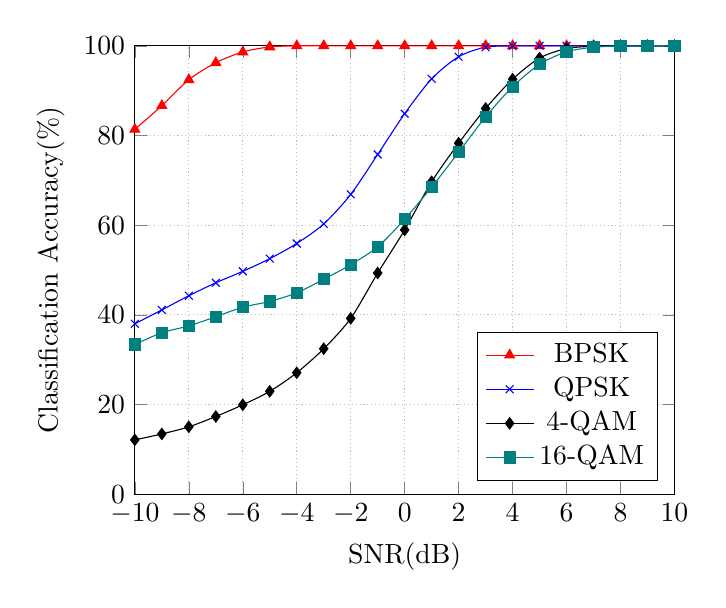
\begin{tikzpicture}
  \begin{axis}[
      xlabel={SNR(dB)},
      ylabel={Classification Accuracy(\%)},
      xmin=-10, xmax=10,
      ymin=0, ymax=100,
      xtick={-10,-8,-6,-4,-2,0,2,4,6,8,10},
      ytick={0,20,40,60,80,100},
      legend pos=south east,
      xmajorgrids=true,
      ymajorgrids=true,
      grid style=densely dotted,
  ]
  \addplot[
      smooth,
      color=red,
      mark=triangle*,
      ]
      coordinates {
      (-10,81.36)(-9,86.65)(-8,92.43)(-7,96.23)(-6,98.62)(-5,99.75)(-4,99.99)(-3,100)(-2,100)(-1,100)(0,100)(1,100)(2,100)(3,100)(4,100)(5,100)(6,100)(7,100)(8,100)(9,100)(10,100)
      };
      \addlegendentry{BPSK}
  \addplot[
      smooth,
      color=blue,
      mark=x,
      ]
      coordinates {
      (-10,37.99)(-9,41.09)(-8,44.25)(-7,47.14)(-6,49.70)(-5,52.53)(-4,55.91)(-3,60.28)(-2,66.86)(-1,75.77)(0,84.86)(1,92.63)(2,97.56)(3,99.69)(4,99.96)(5,100)(6,100)(7,100)(8,100)(9,100)(10,100)
      };
      \addlegendentry{QPSK}
  \addplot[
      smooth,
      color=black,
      mark=diamond*,
      ]
      coordinates {
      (-10,12.10)(-9,13.43)(-8,15.01)(-7,17.32)(-6,19.93)(-5,22.93)(-4,27.08)(-3,32.44)(-2,39.21)(-1,49.32)(0,58.94)(1,69.67)(2,78.27)(3,86.02)(4,92.55)(5,97.27)(6,99.38)(7,99.90)(8,100)(9,100)(10,100)
      };
      \addlegendentry{4-QAM}
  \addplot[
      smooth,
      color=teal,
      mark=square*,
      ]
      coordinates {
      (-10,33.38)(-9,36.00)(-8,37.53)(-7,39.57)(-6,41.70)(-5,42.98)(-4,44.91)(-3,47.93)(-2,51.19)(-1,55.17)(0,61.34)(1,68.49)(2,76.27)(3,84.16)(4,90.86)(5,95.87)(6,98.67)(7,99.67)(8,99.97)(9,100)(10,100)
      };
      \addlegendentry{16-QAM}
  \end{axis}
\end{tikzpicture}
\caption{Classification accuracy of the K-S test classifier with varying noise levels.}
\end{figure}

\begin{figure}[!t]
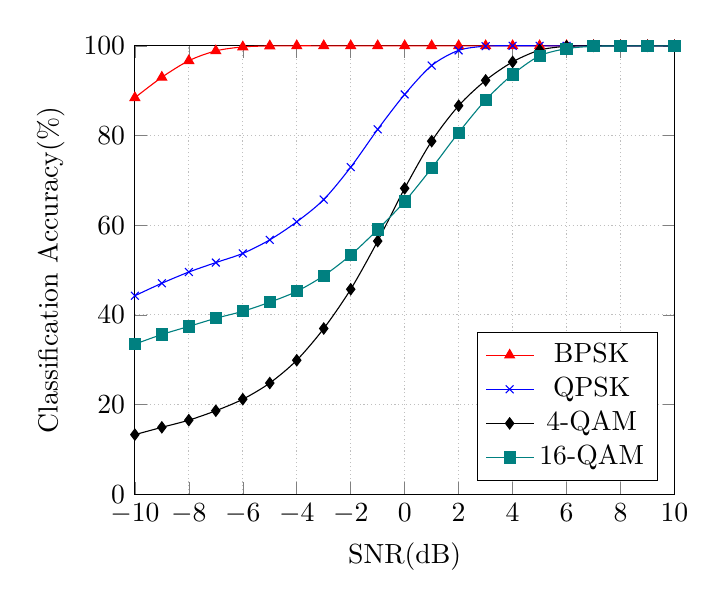
\begin{tikzpicture}
  \begin{axis}[
      xlabel={SNR(dB)},
      ylabel={Classification Accuracy(\%)},
      xmin=-10, xmax=10,
      ymin=0, ymax=100,
      xtick={-10,-8,-6,-4,-2,0,2,4,6,8,10},
      ytick={0,20,40,60,80,100},
      legend pos=south east,
      xmajorgrids=true,
      ymajorgrids=true,
      grid style=densely dotted,
  ]
  \addplot[
      smooth,
      color=red,
      mark=triangle*,
      ]
      coordinates {
      (-10,88.42)(-9,92.98)(-8,96.68)(-7,98.87)(-6,99.75)(-5,99.97)(-4,100)(-3,100)(-2,100)(-1,100)(0,100)(1,100)(2,100)(3,100)(4,100)(5,100)(6,100)(7,100)(8,100)(9,100)(10,100)
      };
      \addlegendentry{BPSK}
  \addplot[
      smooth,
      color=blue,
      mark=x,
      ]
      coordinates {
      (-10,44.25)(-9,47.04)(-8,49.54)(-7,51.65)(-6,53.69)(-5,56.72)(-4,60.74)(-3,65.71)(-2,72.93)(-1,81.37)(0,89.16)(1,95.60)(2,98.98)(3,99.92)(4,100)(5,100)(6,100)(7,100)(8,100)(9,100)(10,100)
      };
      \addlegendentry{QPSK}
  \addplot[
      smooth,
      color=black,
      mark=diamond*,
      ]
      coordinates {
      (-10,13.27)(-9,14.90)(-8,16.50)(-7,18.60)(-6,21.17)(-5,24.78)(-4,29.87)(-3,36.94)(-2,45.70)(-1,56.44)(0,68.21)(1,78.73)(2,86.64)(3,92.29)(4,96.41)(5,99.03)(6,99.89)(7,99.99)(8,100)(9,100)(10,100)
      };
      \addlegendentry{4-QAM}
  \addplot[
      smooth,
      color=teal,
      mark=square*,
      ]
      coordinates {
      (-10,33.45)(-9,35.61)(-8,37.41)(-7,39.22)(-6,40.79)(-5,42.81)(-4,45.23)(-3,48.72)(-2,53.33)(-1,59.02)(0,65.28)(1,72.70)(2,80.64)(3,87.91)(4,93.61)(5,97.76)(6,99.36)(7,99.89)(8,99.98)(9,100)(10,100)
      };
      \addlegendentry{16-QAM}
  \end{axis}
\end{tikzpicture}
\caption{Classification accuracy of the C-v-M test classifier with varying noise levels.}
\end{figure}

\begin{figure}[!t]
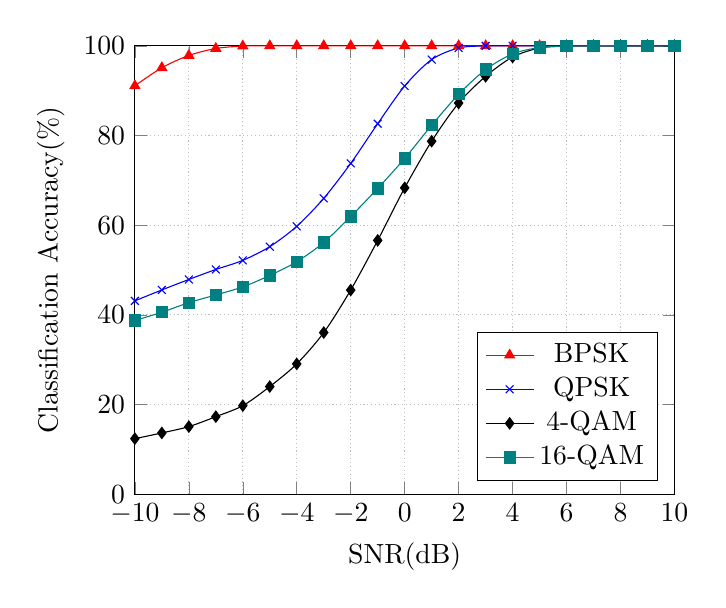
\begin{tikzpicture}
  \begin{axis}[
      xlabel={SNR(dB)},
      ylabel={Classification Accuracy(\%)},
      xmin=-10, xmax=10,
      ymin=0, ymax=100,
      xtick={-10,-8,-6,-4,-2,0,2,4,6,8,10},
      ytick={0,20,40,60,80,100},
      legend pos=south east,
      xmajorgrids=true,
      ymajorgrids=true,
      grid style=densely dotted,
  ]
  \addplot[
      smooth,
      color=red,
      mark=triangle*,
      ]
      coordinates {
      (-10,91.07)(-9,95.11)(-8,97.84)(-7,99.40)(-6,99.94)(-5,99.99)(-4,100)(-3,100)(-2,100)(-1,100)(0,100)(1,100)(2,100)(3,100)(4,100)(5,100)(6,100)(7,100)(8,100)(9,100)(10,100)
      };
      \addlegendentry{BPSK}
  \addplot[
      smooth,
      color=blue,
      mark=x,
      ]
      coordinates {
      (-10,43.11)(-9,45.55)(-8,47.88)(-7,50.11)(-6,52.14)(-5,55.20)(-4,59.74)(-3,65.98)(-2,73.78)(-1,82.63)(0,91.04)(1,96.93)(2,99.52)(3,99.98)(4,100)(5,100)(6,100)(7,100)(8,100)(9,100)(10,100)
      };
      \addlegendentry{QPSK}
  \addplot[
      smooth,
      color=black,
      mark=diamond*,
      ]
      coordinates {
      (-10,12.37)(-9,13.65)(-8,15.06)(-7,17.28)(-6,19.73)(-5,23.99)(-4,29.05)(-3,36.03)(-2,45.53)(-1,56.60)(0,68.32)(1,78.72)(2,87.23)(3,93.19)(4,97.50)(5,99.52)(6,99.95)(7,100)(8,100)(9,100)(10,100)
      };
      \addlegendentry{4-QAM}
  \addplot[
      smooth,
      color=teal,
      mark=square*,
      ]
      coordinates {
      (-10,38.73)(-9,40.57)(-8,42.71)(-7,44.43)(-6,46.23)(-5,48.78)(-4,51.84)(-3,56.13)(-2,61.94)(-1,68.19)(0,74.88)(1,82.28)(2,89.18)(3,94.70)(4,98.2)(5,99.61)(6,99.93)(7,100)(8,100)(9,100)(10,100)
      };
      \addlegendentry{16-QAM}
  \end{axis}
\end{tikzpicture}
\caption{Classification accuracy of the A-D test classifier with varying noise levels.}
\end{figure}

\begin{figure}[!t]
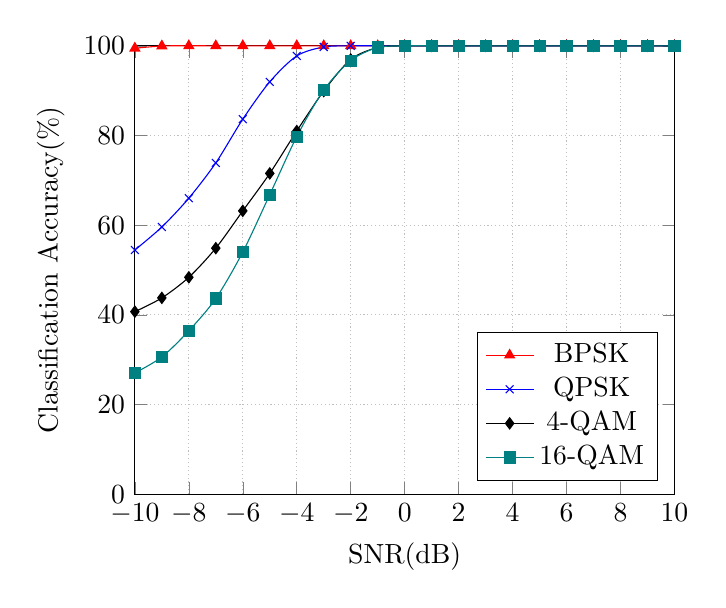
\begin{tikzpicture}
  \begin{axis}[
      xlabel={SNR(dB)},
      ylabel={Classification Accuracy(\%)},
      xmin=-10, xmax=10,
      ymin=0, ymax=100,
      xtick={-10,-8,-6,-4,-2,0,2,4,6,8,10},
      ytick={0,20,40,60,80,100},
      legend pos=south east,
      xmajorgrids=true,
      ymajorgrids=true,
      grid style=densely dotted,
  ]
  \addplot[
      smooth,
      color=red,
      mark=triangle*,
      ]
      coordinates {
      (-10,99.46)(-9,99.96)(-8,100)(-7,100)(-6,100)(-5,100)(-4,100)(-3,100)(-2,100)(-1,100)(0,100)(1,100)(2,100)(3,100)(4,100)(5,100)(6,100)(7,100)(8,100)(9,100)(10,100)
      };
      \addlegendentry{BPSK}
  \addplot[
      smooth,
      color=blue,
      mark=x,
      ]
      coordinates {
      (-10,54.45)(-9,59.59)(-8,66.02)(-7,73.89)(-6,83.64)(-5,91.97)(-4,97.74)(-3,99.74)(-2,100)(-1,100)(0,100)(1,100)(2,100)(3,100)(4,100)(5,100)(6,100)(7,100)(8,100)(9,100)(10,100)
      };
      \addlegendentry{QPSK}
  \addplot[
      smooth,
      color=black,
      mark=diamond*,
      ]
      coordinates {
      (-10,40.70)(-9,43.77)(-8,48.37)(-7,54.87)(-6,63.18)(-5,71.54)(-4,80.99)(-3,89.90)(-2,96.96)(-1,99.61)(0,100)(1,100)(2,100)(3,100)(4,100)(5,100)(6,100)(7,100)(8,100)(9,100)(10,100)
      };
      \addlegendentry{4-QAM}
  \addplot[
      smooth,
      color=teal,
      mark=square*,
      ]
      coordinates {
      (-10,27.03)(-9,30.59)(-8,36.44)(-7,43.63)(-6,54.01)(-5,66.80)(-4,79.73)(-3,90.12)(-2,96.70)(-1,99.62)(0,99.98)(1,100)(2,100)(3,100)(4,100)(5,100)(6,100)(7,100)(8,100)(9,100)(10,100)
      };
      \addlegendentry{16-QAM}
  \end{axis}
\end{tikzpicture}
\caption{Classification of the ML classifier with varying noise levels.}
\end{figure}

\begin{figure}[!t]
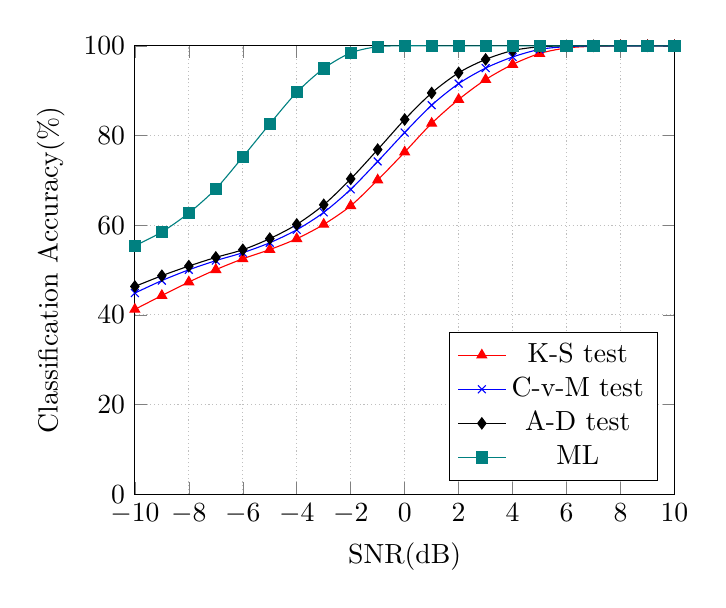
\begin{tikzpicture}
  \begin{axis}[
      xlabel={SNR(dB)},
      ylabel={Classification Accuracy(\%)},
      xmin=-10, xmax=10,
      ymin=0, ymax=100,
      xtick={-10,-8,-6,-4,-2,0,2,4,6,8,10},
      ytick={0,20,40,60,80,100},
      legend pos=south east,
      xmajorgrids=true,
      ymajorgrids=true,
      grid style=densely dotted,
  ]
  \addplot[
      smooth,
      color=red,
      mark=triangle*,
      ]
      coordinates {
      (-10,41.2075)(-9,44.2925)(-8,47.305)(-7,50.065)(-6,52.4875)(-5,54.5475)(-4,56.9725)(-3,60.1625)(-2,64.315)(-1,70.065)(0,76.285)(1,82.6975)(2,88.025)(3,92.4675)(4,95.8425)(5,98.285)(6,99.5125)(7,99.8925)(8,99.9925)(9,100)(10,100)
      };
      \addlegendentry{K-S test}
  \addplot[
      smooth,
      color=blue,
      mark=x,
      ]
      coordinates {
      (-10,44.8475)(-9,47.6325)(-8,50.0325)(-7,52.085)(-6,53.85)(-5,56.07)(-4,58.96)(-3,62.8425)(-2,67.99)(-1,74.2075)(0,80.6625)(1,86.7575)(2,91.565)(3,95.03)(4,97.505)(5,99.1975)(6,99.8125)(7,99.97)(8,99.995)(9,100)(10,100)
      };
      \addlegendentry{C-v-M test}
  \addplot[
      smooth,
      color=black,
      mark=diamond*,
      ]
      coordinates {
      (-10,46.32)(-9,48.72)(-8,50.8725)(-7,52.805)(-6,54.51)(-5,56.99)(-4,60.1575)(-3,64.535)(-2,70.3125)(-1,76.855)(0,83.56)(1,89.4825)(2,93.9825)(3,96.9675)(4,98.9375)(5,99.7825)(6,99.97)(7,100)(8,100)(9,100)(10,100)
      };
      \addlegendentry{A-D test}
  \addplot[
      smooth,
      color=teal,
      mark=square*,
      ]
      coordinates {
      (-10,55.41)(-9,58.4775)(-8,62.7075)(-7,68.0975)(-6,75.2075)(-5,82.5775)(-4,89.615)(-3,94.94)(-2,98.415)(-1,99.8075)(0,99.995)(1,100)(2,100)(3,100)(4,100)(5,100)(6,100)(7,100)(8,100)(9,100)(10,100)
      };
      \addlegendentry{ML}
  \end{axis}
\end{tikzpicture}
\caption{The average classification accuracy of the K-S test, C-v-M test, A-D test and ML classifier with varying noise levels.}
\end{figure}

\begin{table*}[t]
\caption{NUMBER OF OPERATORS NEEDED FOR DIFFERENT CLASSIFIERS USED IN EXPERIMENTS}
\centering
\setlength{\tabcolsep}{5mm}{
\begin{tabular}{cccccc}
\specialrule{0.1em}{3pt}{3pt}
Classifiers & Addition                                    & Multiplier                                 & Logarithm  & Exponential                                & Memory\\
\specialrule{0.1em}{3pt}{3pt}
K-S test    & $MN_{R}(\log_2 N + 2N)$                    & 0                                          & 0          & 0                                          & $MNN_{R}$\\
\specialrule{0em}{3pt}{3pt}
C-v-M test  & $MN_{R}(\log_2 N + 3N)$                    & $NMN_{R}$                                 & 0          & 0                                          & $MNN_{R}$\\
\specialrule{0em}{3pt}{3pt}
A-D test    & $MN_{R}(\log_2 N + 3N)$                    & $2NMN_{R}$                                & 0          & 0                                          & $MNN_{R}$\\
\specialrule{0em}{3pt}{3pt}
ML          & $6NMN_{R}\cdot \sum_{m=1}^{{M}^{N_{T}}}I_m$ & $5NMN_{R}\cdot\sum_{m=1}^{{M}^{N_{T}}}I_m$ & $NMN_{R}$ & $NMN_{R}\cdot \sum_{m=1}^{{M}^{N_{T}}}I_m$ & $MN_{R}$\\
\specialrule{0.1em}{3pt}{3pt}
\end{tabular}}
\end{table*}

In this section, the experiment simulation results are provided to compare the performance of four modulation classifiers with 10,000 realizations of testing signals for each modulation candidate and each SNR varying from -10 dB to 10 dB. Each signal realization consists of 512 observed signal samples at each receiving antenna.
\par The classification performance of various classifiers in AWGN channels for QAM modulations and PSK modulations is shown in Figs. 1-4, respectively. In Fig.~1, the classification results using K-S test classifier are listed for each testing modulation at each noise level. The classification accuracy for BPSK signals achieves 100\% accuracy when SNR is not lower than -3 dB. This robust performance is also displayed in C-v-M test and A-D test classifier, as shown in Fig.~2 and Fig.~3. In terms of overall classification accuracy, the other three modulations are much lower than BPSK at low SNRs particularly. Compared to distribution test classifier shown by Figs.~1-3, the ML classifier achieves better performance at all SNR levels. As we can see from Fig.~4, four modulation signals have achieved excellent performance for SNR = -1dB.
\par Fig.~5 shows the average classification accuracy of different modulation signals based on the proposed classifiers with varying noise levels. It is evident that distribution test classifier is inferior to ML classifier at low SNRs, but they both have robust performance when SNR is higher than 0 dB. The difference in classification accuracy of propsed methods are equal to the ones of ML classifier when SNR is above 6 dB. All of the tested methods reaches near 100\% accuracy about 6 dB.
\par The classification confusion matrices using distribution test based classifiers are shown in Table II for SNR = -4dB. It can be concluded that the BPSK modulation can be recognized most easily. However, the 4-QAM modulation in classification process reflects poor performance by using distribution test classifier.

\subsection{ Complexity Analysis}
To analyze and compare the computational complexity of the proposed four classifiers, the number of mathematical operations required to implement the complete classification process are calculated for each classifier and produced in Table III. Prior to calculating the operation numbers, we first make the following hypotheses: (1) the number of samples of each receiving antenna is $N$, (2) the modulation candidate pool has $M$ number of modulation candidates, (3) the number of receiving antennas is given by $N_{R}$, (4) the number of symbols of the $m$th candidate modulation is represented by $I_m$.
\par From the four tested methods in Table III, we can obviously see that the ML classifier has highest-level computational complexity compared with the other three distribution test methods, which is attributed to the large number of exponential and logarithmic operations needed. Notably, the number of exponential operation scale exponentially with the number of transmitting antennas and modulation order. Such correlation is not found in all three distributiont tests. For a K-S test classifier, it is clear that this has a much lower the computational complexity and only involves addition operation. Addition and multiplier operations are demanded by C-v-M test and A-D test classifier. Moreover, the C-v-M test and A-D test classifier share same number of addition operation. In terms of the system memory, three distribution tests need identical memory and have a much higher memory space than do the ML classifier when received signals $N$ is bigger.

\section{Conclusion}
Three modulation classification techniques based on K-S test, C-v-M test and A-D test have been developed for the MIMO systems. The performance of the proposed algorithms was evaluated in a 2x4 MIMO system with perfect channel knowledge. Three distribution test based classifiers achieve similar classification accuracy. While the performance of proposed distribution test classifiers in AWGN channel is inferior to the popular ML classifier at high noise level, it is of much greater computationally efficient and applicable in sysmtes with higher number of transmitting antennas and modulation order.
% use section* for acknowledgment

% Can use something like this to put references on a page
% by themselves when using endfloat and the captionsoff option.
\ifCLASSOPTIONcaptionsoff
  \newpage
\fi



% trigger a \newpage just before the given reference
% number - used to balance the columns on the last page
% adjust value as needed - may need to be readjusted if
% the document is modified later
%\IEEEtriggeratref{8}
% The "triggered" command can be changed if desired:
%\IEEEtriggercmd{\enlargethispage{-5in}}

% references section

% can use a bibliography generated by BibTeX as a .bbl file

% BibTeX documentation can be easily obtained at:
% http://mirror.ctan.org/biblio/bibtex/contrib/doc/
% The IEEEtran BibTeX style support page is at:
% http://www.michaelshell.org/tex/ieeetran/bibtex/
%\bibliographystyle{IEEEtran}
% argument is your BibTeX string definitions and bibliography database(s)
%\bibliography{IEEEabrv,../bib/paper}
%
% <OR> manually copy in the resultant .bbl file
% set second argument of \begin to the number of references
% (used to reserve space for the reference number labels box)
\begin{thebibliography}{00}

\bibitem{Choqueuse2009}
V. Choqueuse, S. Azou, K. Yao, L. Collin, and G. Burel, ``Blind Modulation Recognition for MIMO Systems,'' Milit. Tech. Acad. Rev., vol. XIX, no. 2, pp. 183--196, 2009.
\bibitem{Kanterakis}
E. Kanterakis and W. Su, ``Modulation Classification in MIMO Systems,'' in 2013 IEEE Milit. Commun. Conf.(MILCOM) San Diego, CA, pp. 35--39, 2013.
\bibitem{Muhlhaus}
M. S. Muhlhaus, M. Oner, O. A. Dobre, and F. K. Jondral, ``A Low Complexity Modulation Classification Algorithm for MIMO Systems,'' in IEEE Commun. Lett., vol. 17, no. 10, pp. 1881--1884, 2013.
\bibitem{Abu-Romoh}
M. Abu-Romoh, A. Aboutaleb, and Z. Rezki, ``Automatic Modulation Classification Using Moments and Likelihood Maximization,'' in IEEE Commun. Lett., vol. 22, no. 5, pp. 938--941, 2018.
\bibitem{Zhang}
K. Zhang, E. L. Xu, Z. Feng, and P. Zhang, ``A Dictionary Learning Based Automatic Modulation Classification Method,'' in IEEE Access, vol. 6, pp. 5607--5617, 2018.
\bibitem{Ali}
A. Ali and F. Yangyu, ``Automatic Modulation Classification Using Deep Learning Based on Sparse Autoencoders With Nonnegativity Constraints,'' in IEEE Signal Process. Lett., vol. 24, no. 11, pp. 1626--1630, 2017.
\bibitem{Wu}
Z. Wu, S. Zhou, Z. Yin, B. Ma, and Z. Yang, ``Robust Automatic Modulation Classification Under Varying Noise Conditions,'' in IEEE Access, vol. 5, pp. 19733--19741, 2017.
\bibitem{Wang}
F. Wang and X. Wang, ``Fast and robust modulation classification via Kolmogorov–Smirnov test,'' IEEE Trans. Commun., vol. 58, no. 8, pp. 2324--2332, 2010.
\bibitem{Zhu}
Z. Zhu, M. W. Aslam, and A. K. Nandi, ``Genetic algorithm optimized distribution sampling test for M-QAM modulation classification,'' Signal. Proc., vol. 94, pp. 264--277, 2014.
\bibitem{Kolmogorov}
J. Frank and J. Massey, ``The Kolmogorov-Smirnov Test for Goodness of Fit,'' J. Am. Stat. Assoc., vol. 46, No. 253, pp. 68--78, 1951.
\bibitem{Cramer}
 H. Cramer, ``On the Composition of Elementary Errors,'' Sc. Act. J., vol. 1, pp. 13--74, 1928.
\bibitem{Anderson}
T. W. Anderson and D. A. Darling, ``A Test of Goodness of Fit,'' J. Am. Stat. Assoc., vol. 49, No. 268, pp. 765--769, 1954.
\bibitem{Laio}
F. Laio, ``Cramer--von Mises and Anderson-Darling goodness of fit tests for extreme value distributions with unknown parameters,'' Water. Res. R., vol. 40, no. 9, pp. 1--10, 2004.
\end{thebibliography}

% biography section
%
% If you have an EPS/PDF photo (graphicx package needed) extra braces are
% needed around the contents of the optional argument to biography to prevent
% the LaTeX parser from getting confused when it sees the complicated
% \includegraphics command within an optional argument. (You could create
% your own custom macro containing the \includegraphics command to make things
% simpler here.)
%\begin{IEEEbiography}[{\includegraphics[width=1in,height=1.25in,clip,keepaspectratio]{mshell}}]{Michael Shell}
% or if you just want to 如何使用.cls .tex文件reserve a space for a photo:


% \end{IEEEbiography}if you will not have a photo at all:

% insert where needed to balance the two columns on the last page with
% biographies
%\newpage

% You can push biographies down or up by placing
% a \vfill before or after them. The appropriate
% use of \vfill depends on what kind of text is
% on the last page and whether or not the columns
% are being equalized.

%\vfill

% Can be used to pull up biographies so that the bottom of the last one
% is flush with the other column.
%\enlargethispage{-5in}



% that's all folks
\end{document}
